\textbf{ODMR} is a resonance technique by which the electron of a crystal 
defect may be optically excited and its spin state will initialized by the 
spin selection and readout. Among other materials this a method most 
frequently used on diamond has nitrogen vacancy defects (NV). Yet, it is
quite hard to find a comprehensive and clear explanation of the method 
including application details. Here, I will provide detailed information on
our measurement and data processing methods for measuring the ODMR contrast.

\subsection{Data acquisition and initial processing}
Since ODMR method relies on the observation of changes in the PL emission 
spectra of the target material defects, it requires either a spectrometer 
or a photon counting unit like PMT or APD. Our setup utilizes a relatively 
low-profile and low-cost spectrometer from ASEQ Instruments[ref here!!] for
the collection of PL emission. The PL emission from NV diamond is basically  
coupled in to the spectrometer through an optical fiber as it was shown in 
Figure\ref{fig:ConfocalReflectingMicroscopeFull}. This is the raw PL data 
which depending on the setup includes dark background counts produced in the
detector chip, fluorescence background emission produced by the buffer media
where the actual sample resides, and the actual PL emission from the target
material, here NV defects in the diamond. Identification of these emissions 
from different sources and isolation of the PL from NV defects are imperative
for proper quantification ODMR data.

\subsubsection{Spectrometer properties and dark background counts}\label{subsubsec:darkBGMethod}
Typically a spectrometer is a device which reads out photon counts based on
the wavelength. To accomplish that input light is coupled to the device either
through air or an optical fiber. Within a spectrometer the input light 
shines on to a grating and diffracted, based on its wavelength. Spatially 
split photons hit to a silicone line detector (charge coupled device, aka. 
CCD). These photons create electrons on the chip units/pixels and read as
the counts acquired per pixel. 

ASEQ spectrometer has the line detector TCD1304DG from Toshiba as its sensor.
This is a 3694 pixel detector and 3654 of them are set to be used in a measurement.
Currents from CCD are converted to photon counts per pixel through a 16 bit
analog to digital converter (ADC). Therefore the maximum counts per pixel
is limited to 65535. A CCD is know to generate photon counts even the absence 
of input light which is called dark counts or dark background of the CCD.


On typical an upright or inverted microscope, illumination light comes from a direction 
relative to sample surface, while the collection or imaging is done in the opposite direction. 
Therefore in terms of optical components, illumination and imaging sides differ in those
systems. For example in illumination side a special lens called \textbf{Condenser} focuses
the light on to the sample while in the imaging side another special lens called \textbf{
Objective} lens collects the light coming from the sample. These special lenses and the
typical upright and inverted microscope configurations are shown in Figure\ref{fig:CondenserAndObjective}.

%\begin{figure}[H]
%	\centering
%	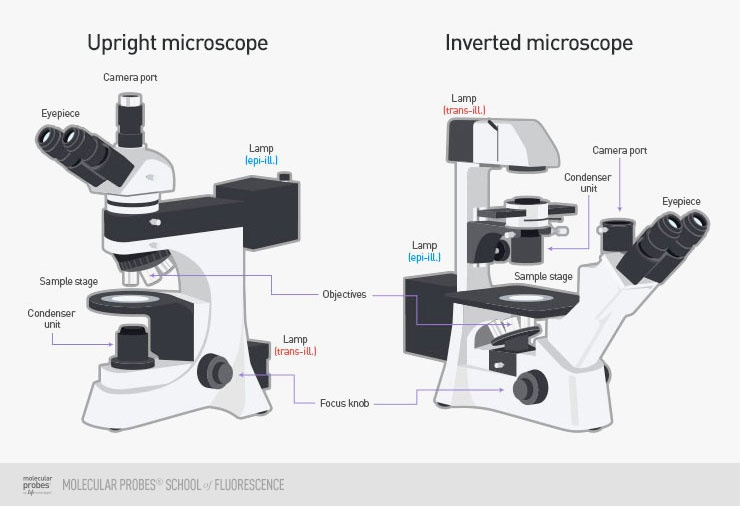
\includegraphics[angle=0,origin=c,width = 1.0\linewidth]{Section_Microscope/Figures/CondenserAndObjective.jpg}
%	\caption{A typical upright (\textbf{left}) and an inverted (\textbf{right}) microscope 
%		structures indicating the positions of special lenses (\textbf{Condenser and objective}).}
%	\label{fig:CondenserAndObjective}
%\end{figure}
%
%On the other hand, in a reflecting microscope illumination and imaging are done through the
%same optical path or by same optics. As it is shown in Figure\ref{fig:ReflectingMicroscope},
%shared optical path allows one (1) additional port for imaging and/or illuminating the sample
%on a typical reflecting microscope. This port is very frequently assigned to white-light
%(\textbf{bright-field}) imaging through a camera, so it is called the camera port. As a result
%any additional illumination and/or imaging on top of the default system, require a custom
%design optical system with the ability to finely couple with the existing microscope.
%
%\begin{figure}[H]
%	\centering
%	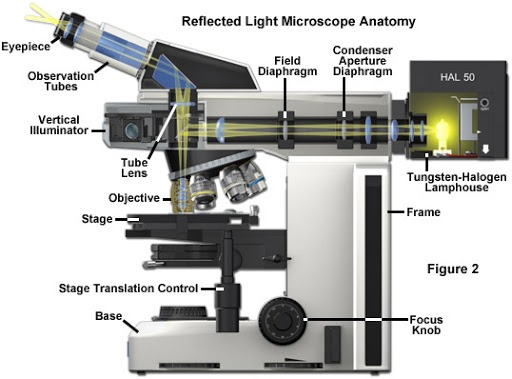
\includegraphics[angle=0,origin=c,width = 1.0\linewidth]{Section_Microscope/Figures/ReflectingMicroscope.jpeg}
%	\caption{Schematics of a typical reflecting microscope with light path and internal 
%		optical components.}
%	\label{fig:ReflectingMicroscope}
%\end{figure}
%
%\subsection{Confocal Systems Overview}\label{sec:confocalsystems}
%A \textbf{confocal system} is an imaging system that utilizes a spatial filter
%(or simply a pinhole) before the imaging component for strictly matching the illumination 
%volume with the observation volume as it is shown in Figure\ref{fig:WidefieldVsConfocal}. Because 
%of very likely chromatic aberrations \footnote{\url{https://www.microscopyu.com/tutorials/chromatic}} 
%through the imaging components, usually illumination is done by a single color light source such as 
%a laser. The pinhole suppresses the out-of-excitation volume light dramatically, so it increases 
%the resolution of imaging system, Figure\ref{fig:WidefieldVsConfocalResolution}. REF HERE!!!!
%
%\begin{figure}[H]
%	\centering
%	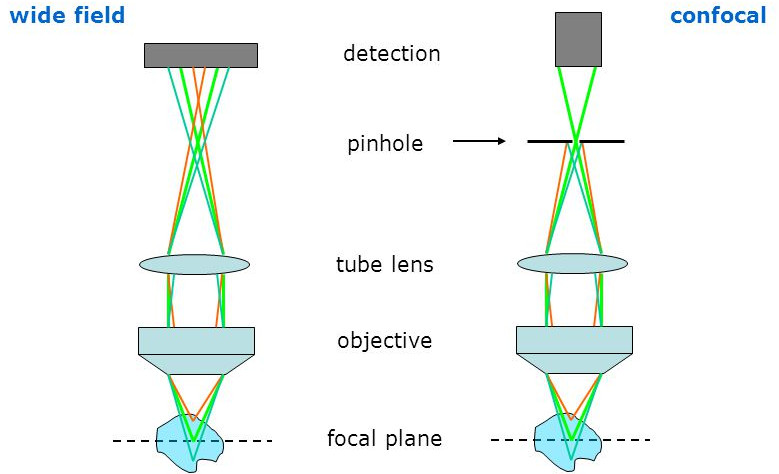
\includegraphics[angle=0,origin=c,width = 1.0\linewidth]{Section_Microscope/Figures/Confocal_microscopy_Basic_principle1.jpg}
%	\caption{Simplified structure of a typical widefield (\textbf{left}) and a confocal (\textbf{right})
%		imaging system  with spatial filter. ADD REF-FOOTNOTE HERE!!!}
%	\label{fig:WidefieldVsConfocal}
%\end{figure}
%
%\begin{figure}[H]
%	\centering
%	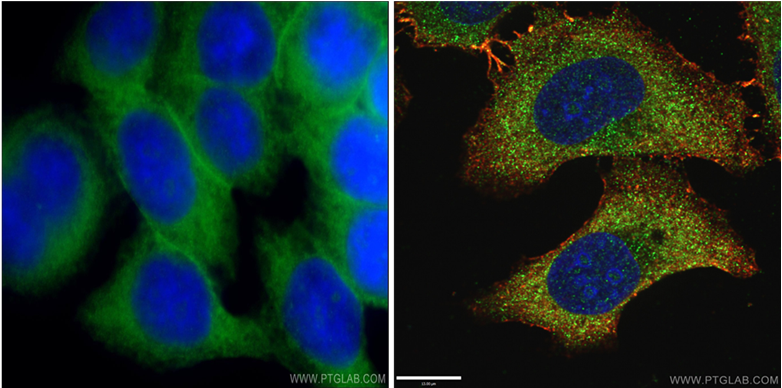
\includegraphics[angle=0,origin=c,width = 1.0\linewidth]{Section_Microscope/Figures/EpiVsConfocal1.png}
%	\caption{Imaging of HeLa cells with a typical widefield (\textbf{left}) and with a confocal 
%		(\textbf{right}) imaging system. ADD REF-FOOTNOTE HERE!!!}
%	\label{fig:WidefieldVsConfocalResolution}
%\end{figure}
%
%Microscope manufacturers very frequently incorporate additional openings (called \textbf{microscope ports})
%on sides, front and even at the bottom of microscope bodies which allows the operator to 
%couple additional imaging and illumination systems into the microscope. Although this is 
%a very common practice in the case of transmission microscopes (upright and inverted as well),
%reflecting microscopes usually don't have these additional ports, Figure\ref{fig:ReflectingMicroscope}. 
%Because of missing ports, turning a reflecting microscope is considerably harder into 
%a confocal system compared to transmission microscopes. 
%
%\subsection{Confocal Reflecting Light Microscope for PL Measurements}
%
%Our goal is to observe emission from excited lattice-defects in solids like boron 
%nitride(BN) and diamond[REF HERE!!!]. These materials are not particularly transparent
%to visible light\footnote{\url{https://en.wikipedia.org/wiki/Boron_nitride}}. Moreover
%defect formation (particularly in the case of BN) is induced by ion bombardment, so
%neither the density nor spatial distribution of defects are known prior to a PL 
%measurement. The lack of information on defect positions introduces the requirement 
%of active search for defects within the sample volume, so a confocal imaging system 
%with the capability of scanning. To overcome the refractive index issue and satisfying 
%the confocality in imaging, we built a confocal reflecting light microscope as shown
%in Figure\ref{fig:ConfocalReflectingMicroscopeFull}.
%
%\begin{figure}[H]
%	\centering
%	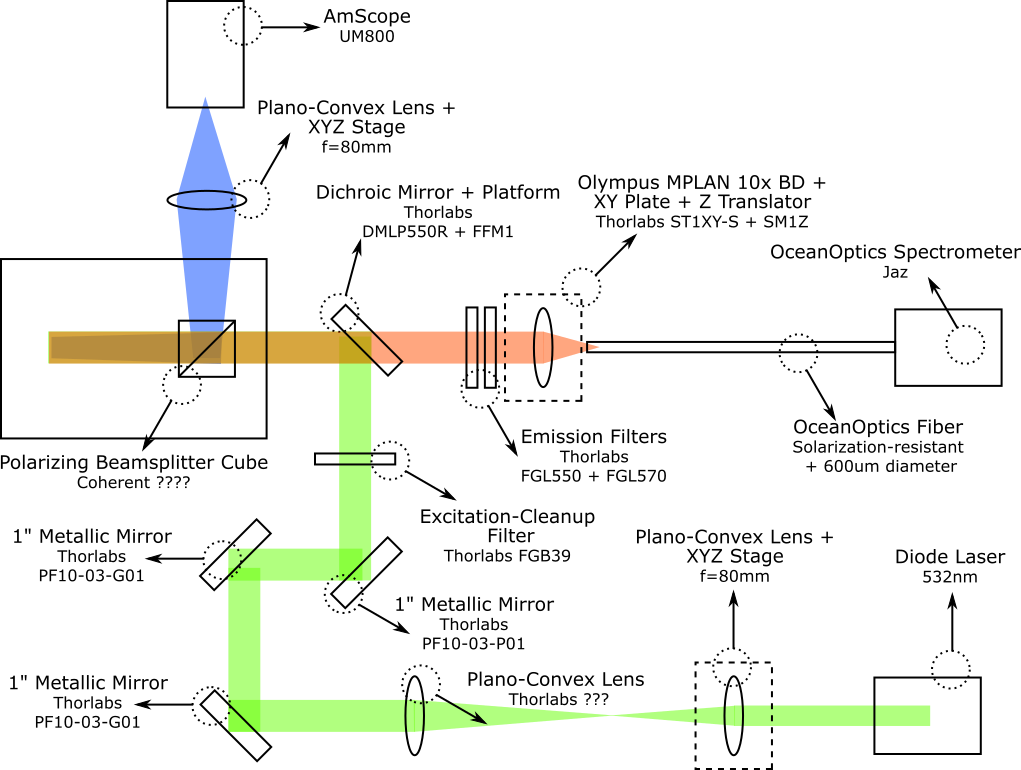
\includegraphics[angle=0,origin=c,width = 0.95\linewidth]{Section_Microscope/Figures/PL_Setup_Parts.png}
%	\caption{Our homemade confocal reflecting microscope for PL measurements.}
%	\label{fig:ConfocalReflectingMicroscopeFull}
%\end{figure}
%
%Although the purpose of individual parts can not be explained accurately by ignoring their 
%interactions with the remaining system components, it is a common practice to divide the whole 
%system into 4 essential zones for educational purposes as in Figure\ref{fig:ConfocalReflectingMicroscopeZones}. 
%
%\begin{figure}[H]
%	\centering
%	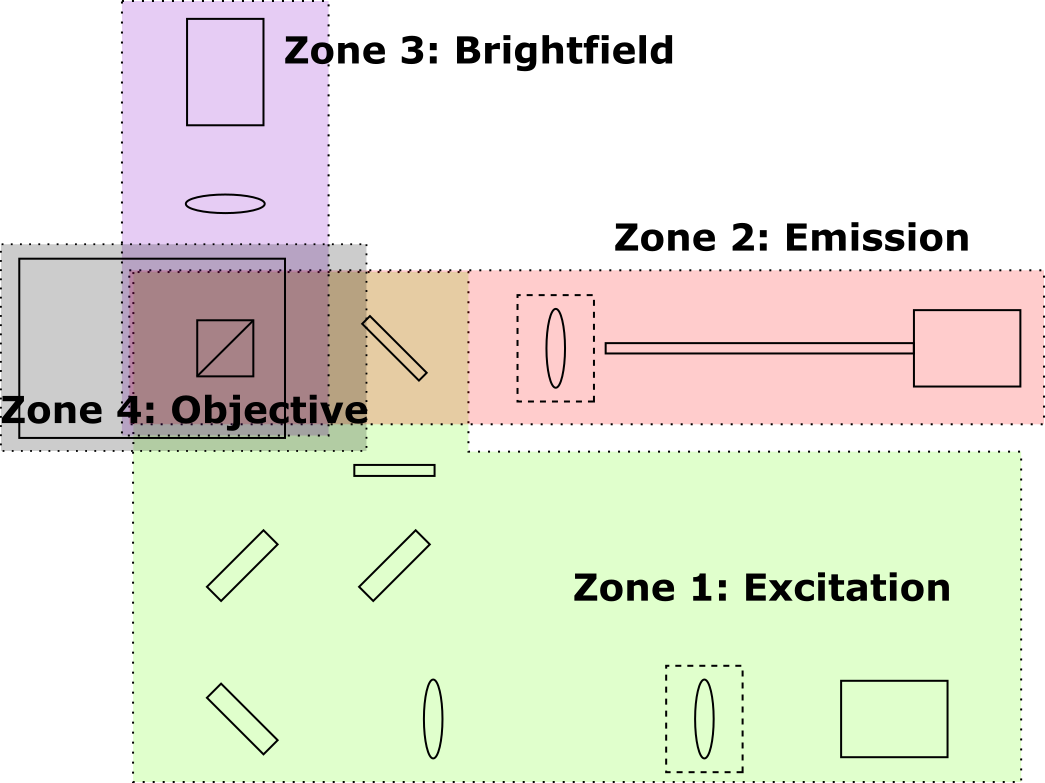
\includegraphics[angle=0,origin=c,width = 0.95\linewidth]{Section_Microscope/Figures/PL_Setup_Zones.png}
%	\caption{Zones in PL microscope.}
%	\label{fig:ConfocalReflectingMicroscopeZones}
%\end{figure}
%
%To briefly describe these zones;
%
%\begin{enumerate}
%	\item \textbf{Excitation, Zone 1 :} This is the zone where the excitation light is directed 
%	into the microscope. The excitation source is frequently a laser, but there are systems
%	which prefer broadband light sources such as UV lamps. In this zone, beam characteristics
%	of excitation light (i.e. size, divergence, polarization, etc.) are adjusted to match the
%	requirements imposed by other zones.
%
%	\item \textbf{Emission, Zone 2 :} This is the zone where the emission or reflection from
%	the sample is collected and analyzed by a detector. The detector can be any photon sensitive
%	device (i.e. PMT, APD, CCD camera, etc.). Based on the preferred coupling mechanism in the
%	sensory device, characteristics of the emission from the sample are adjusted similar to the 
%	case the adjustment of excitation light.
%	
%	\item \textbf{Brightfield, Zone 3 :} This is the zone responsible to visual inspection of
%	the sample surface and excitation/emission light profiles on the sample. Its mere purpose is
%	to create an image of the sample surface and everything in near proximity on a camera and 
%	allow guided tracking.
%	
%	\item \textbf{Objective, Zone 4 :} This is the zone where the primary imaging lens called
%	objective lens resides. As a result, it is the core of the whole optical system and couples
%	with all other zones. In other words, optical components in other zones are chosen/built 
%	essentially for matching the objective lens to utilize the whole measurement system at its 
%	maximum efficiency.
%\end{enumerate}
%
%As in any other optical system, efficiency of imaging in this system is strongly correlated with
%match ratio of all these zones. Although it appears to be the Objective (Zone) 4 is the central
%piece that all other zones required to be matched, there are matching requirements for among other
%zones too. As a result, proper description of the microscope require deeper understanding of all
%zones.
%
%\subsubsection{Excitation, Zone 1}\label{subsubsec:excitationCouplings}
%In terms of the structure, this zone directly couples into Objective (Zone 4) and indirectly couples 
%into Emission (Zone 2). In terms of the alignment, it directly couples into Brightfield (Zone 3).
%These couplings and the required matching conditions are as following;
%
%\paragraph{Direct structural coupling between Excitation and Objective Zones}\mbox{}\\
%This coupling is dictated by the three essential \textbf{optical design rules};
%
%\begin{enumerate}
%	\item \ul{Excitation light going into the Objective has to be collimated}, so it should not be
%	converging or diverging in free space for a long enough distance. On the other hand, the level of 
%	collimation is very frequently not perfect, because of the real/non-ideal objective lenses.
%	To address this we placed a telescope in the path of excitation light as shown in the Figure
%	\ref{fig:ConfocalReflectingMicroscopeFull}. In addition, the first lens in the telescope is 
%	positioned on a XY-stage to finely tune the convergence/divergence of the excitation light.
%	
%	\item \ul{Propagation direction of the incoming light to the objective lens has to be 
%	parallel with the surface normal of the objective lens}. A well aligned excitation beam 
%	removes undesired distortions in the structure of focused light after the objective lens.
%	This is addressed by introducing two 1" mirrors to the light path right before the excitation-
%	cleanup filter. As it is shown in the Figure\ref{fig:ConfocalReflectingMicroscopeFull},
%	the mirror closest to the filter is responsible for angular change while the one before
%	that mirror is responsible for translation of the excitation beam, both relative to the
%	objective lens' surface normal.
%	
%	\item \ul{The ratio of the diameter of excitation light and the diameter of back-aperture of the 
%	objective lens (\textbf{aperture filling ratio}) has to be known and fixed to a value} 
%	depending on the experimental needs (i.e. tight focus, scanning beam, etc.). previously mentioned
%	telescope not only sets the angular dispersion of the laser but it also adjusted the beam diameter.
%	By using a ~200mm focal lens in the telescope, we set the beam diameter slightly larger than 
%	the back-aperture of the objective lens.
%\end{enumerate}
%
%\paragraph{Indirect structural coupling between Excitation and Emission Zones}\mbox{}\\
%This coupling is dictated by the confocality of the system. To be more precise, while excitation
%zone is describing the input excitation beam, it also defines the distance and size of the
%focused beam on the front-focal plane of the objective lens. As it was indicated in Section
%\ref{sec:confocalsystems}, spatial filter (pinhole) position and its size has to be adjusted
%according to the focus position and size. 
%
%\paragraph{Direct alignment coupling between Excitation and Brightfield Zones}\mbox{}\\
%In the case of a conventional microscope, optics in the brightfield zone need to be aligned
%prior to sending additional input light. This is called K\"{o}hler illumination
%\footnote{\url{https://www.olympus-lifescience.com/en/microscope-resource/primer/anatomy/kohler/}}
%which is not fully implemented in our microscope. Instead we illuminate the sample surface with
%a ring of LEDs around the objective lens housing and collect the reflecting light either with
%a camera or with an additional long focal length lens. Purpose of the long focal length lens is 
%for the adjustment of field of view (FOV\footnote{\url{https://www.edmundoptics.com/knowledge-center/
%		application-notes/imaging/understanding-focal-length-and-field-of-view/}}). Therefore
%before adjusting the focal position of the laser in the front focal plane of the objective lens,
%we try to see the image of the sample surface. Once a clear image is observed, we adjust the 
%convergence/divergence of the laser beam to place the laser focus on to the image plane.
%
%\subsubsection{Emission, Zone 2}\label{subsubsec:emissionCouplings}
%In terms of the structure, this zone directly couples into Objective (Zone 4) and indirectly couples 
%into Excitation (Zone 1). In terms of the alignment, it directly couples into Brightfield (Zone 3).
%These couplings and the required matching conditions are as following;
%
%\paragraph{Direct structural coupling between Emission and Objective Zones}\mbox{}\\
%This coupling is dictated by the objective lens being non-ideal or real. [ADD A PICTURE!!!].
%Even though microscope objectives are called infinity-corrected\footnote{\url{https://
%		www.olympus-ims.com/en/microscope/terms/feature15/}}, like all real lenses they have 
%two focal planes namely back (BFP) and front (FFL) focal planes \footnote{\url{https://
%		en.wikipedia.org/wiki/Cardinal_point_(optics)}}. A confocal system uses BFL of the 
%objective lens or its image to spatially filter the emission. In our system the fiber optics 
%cable is used to spatially filtering the emission at a proper position where there is the first
%image of BFL is formed.
%
%\paragraph{Indirect structural coupling between Emission and Eexcitation Zones}\mbox{}\\
%Although this coupling is explained in Excitation section, it is worth mentioned that apart
%from the coupling through objective lens' focal plane positions Excitation Zone sets the 
%operable size range for spatial filter by defining the excitation beam profile. The coupling
%considered to be crucial for the resolution of the whole microscope, so a very detailed work
%is provided in literature.[REF HERE!!!]
%
%\paragraph{Indirect alignment coupling between Emission and Brightfield Zones}\mbox{}\\
%Although this coupling is explained in Excitation section, it is worth mentioned that apart
%from the coupling through objective lens' focal plane positions Excitation Zone sets the 
%operable size range for spatial filter by defining the excitation beam profile. The coupling
%considered to be crucial for the resolution of the whole microscope, so a very detailed work
%is provided in literature.[REF HERE!!!]
%
%\subsubsection{Brightfield, Zone 3}\label{subsubsec:brightfieldCouplings}
%Given that this zone's couplings with Excitation and Emission zones are already presented in
%sections \ref{subsubsec:excitationCouplings} and \ref{subsubsec:emissionCouplings}, its
%remaining coupling is with the Objective (Zone 4). 
%
%\paragraph{Direct structural coupling between Brightfield and Objective Zones}\mbox{}\\
%A proper brightfield image of the sample plane means that an image formed on the CCD camera
%chip with minimal optical aberrations\footnote{\url{https://www.edmundoptics.com/knowledge-center/
%		application-notes/optics/comparison-of-optical-aberrations/}}. Among which chromatic aberration, 
%field curvature, distortion, and defocus are the ones frequently observed in homemade systems.
%
%\begin{itemize}
%	\item There is not a perfect solution for chromatic aberration because it is related with 
%	the objective lens' response to excitation and emission wavelengths. Objective lenses are 
%	quite a bit expensive instruments and it is highly unlikely that a research group can
%	effort purchasing unique objective lenses for individual experiments. As a result, a 
%	partial solution for chromatic aberration is  to image the excitation light focus and
%	the sample surface within the range of operable wavelengths.
%
%	\item Defocus and distortion are the ones related with the relative axial positions of 
%	the objective lens, camera lens, and the camera. These aberrations are required to be 
%	corrected by altering lens and camera positions in an ad-hoc fashion on the light 
%	propagation axis. It is also useful to have an imaging lens of similar focal length 
%	to tube lens of objective lens was designed for.
%
%	\item Field curvature occurs by the mismatch between objective lens and the remaining
%	lens(es) in the imaging pathway. It is highly likely that the image forming lens for
%	camera is not exactly same as actual tube lens in a commercial microscope. As a result
%	it is very likely that outer edges of the image will be distorted in a homemade system.
%	As long as the desired portion of the image around center is good enough, there is no
%	need to put extra effort to find an exact copy of tube lens.
%\end{itemize}
%
%\subsubsection{Objective, Zone 4}
%Coupling of Objective (Zone 4) with other zones are covered in sections \ref{subsubsec:excitationCouplings},
%\ref{subsubsec:emissionCouplings}, and \ref{subsubsec:brightfieldCouplings}. 
